\documentclass[12pt,a4paper]{article}
\usepackage[top=1in, bottom=1in, left=1.25in, right=0.75in]{geometry}
\usepackage{mdwlist}
\usepackage{hyperref}
\usepackage{amssymb}
\usepackage{graphicx}
\usepackage{float}
\usepackage{url}
\usepackage{setspace}
\usepackage{amsmath,amsthm,amssymb}
\usepackage[procnames,noindent]{lgrind}

\hypersetup{colorlinks=false,pdfborder={0 0 0}}
\begin{document}
\thispagestyle{empty}
\tableofcontents
\newpage

\section{Chapter : INTRODUCTION}
\onehalfspacing
\ \ \ \ Sudoku ‎is a \textit{mathematical, logical and permutational puzzle} which contains 9x9 grid of cells. Each of nine row, column and box (3x3) grid contains value from 1-9 without any repetitions. Using these properties one can try solving the puzzle. Puzzle is said to be solved if the entire 9x9 cells are filled with values with out any conflicts (any value repetiting in the same row, coloumn or box). There any many types of sudokus. Generic sudoku (the one discussed below and the most widely used), word sudoku, 
Jigsaw or Squiggle Sudoku, samurai sudoku etc. 

\begin{figure}[H]
\begin{center}
\ \newline
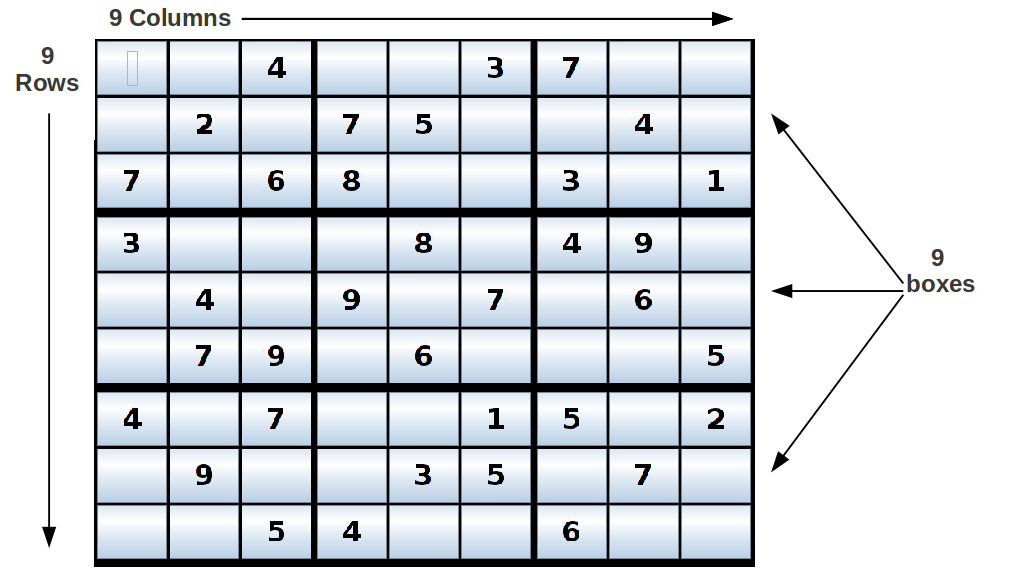
\includegraphics[scale=.5]{typicalsudoku.png}
\caption{Typical Sudoku example}
\end{center}
\end{figure}


\subsection{Aim / Objective}
\ \ \ \ The main endeavor of this project is to find a mathematical solution for solving sudoku.  There exist many algorithms for generating sudokus, but not for solving them (only few exist). Hence we give a computerized solution to sudoku. The technique discussed in this report is a new approach which tries to reduce the space and time complexity with still having ability solve sudoku. The technique uses \textbf{SET Operations} to solve sudoku. This approach also determines whether a sudoku is solvable \textit{without guess} or \textit{not}.
\ \newline

\subsection{Existing System}
\ \ \ \ As specified earlier there exist many system which efficiently generate sudokus of different levels (easy, hard etc), but there are only few techniques which concentrate on providing solution to them. This is because it is generated so that it can be solvable by humans. But there are ceratain sudokus which require guess and are complex to solve. The traditional approaches were in the \textbf{\textit{O( n$^n$)} (backtracking) or \textit{O(n$^5$)} (brute force techniques)}. These approaches have high time and space complexities. As there are only few techniques for solving sudoku, there is a lot of scope for new approaches for solving sudoku with having lower space and time complexities. 

\newpage
\section{Chapter: Propsed System}
\ \ \ \ The system proposed uses \textit{\textbf{SET operations}} to solve sudoku. In this approach the main endeavor is to reduce the space and time complexity of the algorithms. A new Data Structures for SET is designed so that it reduces the complexities. Set operations such as \textit{Union, Intersection, Difference, Compliment} are implemented. These set operations are applied on the cells of the sudoku to determine the values to be filled in these cells. The Set Data Structure is implemented using \textbf{\textit{BitVectors}}. BitVector is another Data structure which uses only few bits to hold certain values and it best suits for implementing SET Data Structure. 

\subsection{Why sets?}
\ \ \ \ The properties of Sodoku such as \textit{\textbf{``No Repetition"}} of values in row, column and box and each of the cells can have a \textit{\textbf{``Set"}} of possible values which can appear in the cell (because the order of the possible values does not matter). It is obvious that if a cell has a possible values `x' and if it does not appear as a possible value in any of the other cell in the same box then `x' can be filled in that cell. Determining such things can be easily done using \textit{``union and difference"}. SETs are one of the important fields of discrete mathematics. Though it is not widely used in applications, but still has its own importance. Using SETs as a tool for solving Sudoku increases the efficiency and elegance. 

\subsection{Introduction to BitVectors}
\ \ \ \ \textit{\textbf{``BitVectors"}} is a Data Structure created specifically for implementing `SET' and its associated operations. The importance of the Data Structure to solve a problem can be realized in \textit{BitVectors}. As Sudoku can have a maximum of 9 digits the \textit{Union}, \textit{Intersection} and \textit{Difference} can be implemented in \textit{\textbf{O(1)}}. BitVector can be considered as a linked list of bits corresoponding to a particular number. \textit{\textbf{Base}} represents the base value to the node and the \textit{\textbf{9-bits}} repressent nine numbers starting from \textit{Base}. i.e., if a bit \textit{`i'} is set then a number \textit{`i' + `Base'} exists. For e.g. Consider base value as `1' and a 5$^{th}$ bit is set then a number `5' exists in the set. It also contains a pointer which point to the next node in the list of BitVector. 

\begin{figure}[H]
\begin{center}
\ \newline
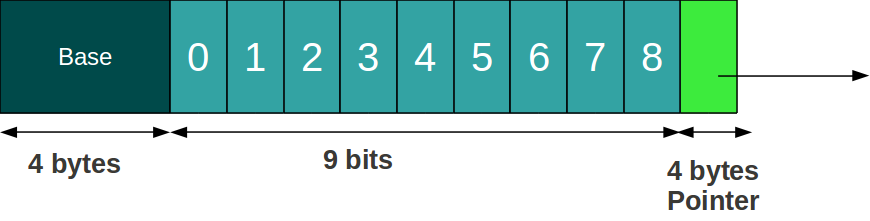
\includegraphics[scale=.4]{bitvector.png}
\caption{Representation of BitVector}
\end{center}
\end{figure}

\subsection{Advantages of BitVector}
\ \ \ \ Specific to this application only a single node with 9-bits are used. This representation of data structure is important inorder to reduce the space and time complexity. If we want to store 9 values and decide the represent it in an array then it requres 9 positions in memory and each of which would requre 4 bytes. So totally the array representation requires \textbf{9x4=36} bytes, where as BitVector Requres only \textbf{8 bytes plus 1 bit} which is saves around \textbf{77.5\%} of space. We know that implementing Union, intersection and difference in an array is of \textbf{O(n$^2$)}.  But the main advatange of BitVector lies here. \textbf{BitVectors implement the SET operation in \textit{O(1)}}. Let us see how BitSets implement Set operations in \textit{O(1)}.

\subsection{Implementation details of Union ($\bigcup$) operation}
\ \ \ \ The figure 3 illustrates how \textit{\textbf{union}} operation is implemented in O(1) using BitVectors with the help of \textbf{\textit{OR}} operation. As we know that union of two sets would result in a set which includes all the elements in both the sets and the repeated values are eliminated, similarly when we perform OR operation, if bits in two corresponding BitVectors are set, then the resulting BitVector will also have the same correspoding bit set, so it is counted only once. So to perform Union of two BitVectors it requires only one \textit{OR} operation.
\begin{figure}[H]
\begin{center}
\ \newline
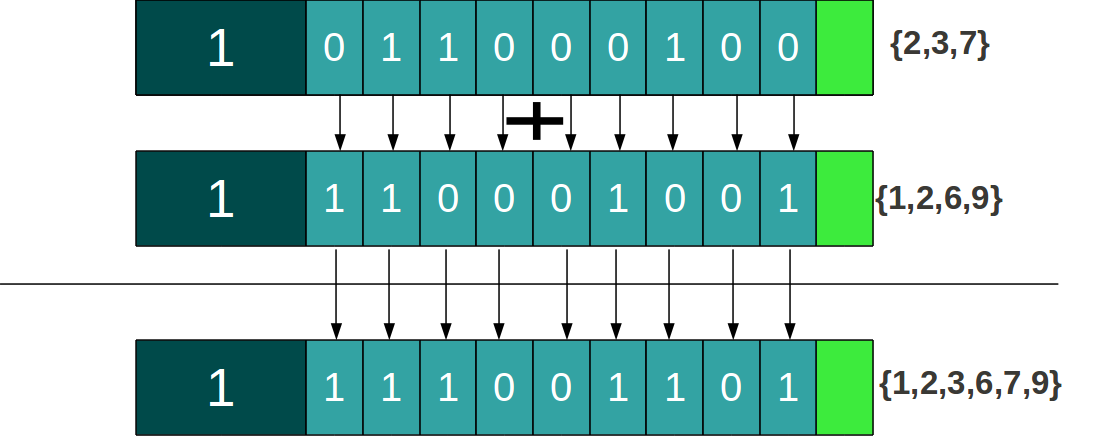
\includegraphics[height=50mm, scale=.5]{union.png}
\caption{Union operation achieved by OR-ing two BitVectors}
\end{center}
\end{figure}

\subsection{Implementation details of Intersection $(\bigcap)$ operation}
\ \ \ \ The figure 4 illustrates how \textit{\textbf{intersection}} opreation is implemented in O(1) using BitVectors with the help of \textit{\textbf{AND}} oeration. \textit{Intersection} of two sets would result in a set which would include elements which are there in both the sets. To achieve this \textit{AND} operation is performed on the two BitVectors. If corresponding bits in both the BitVectors are set then only the corresponding bit in the resultant BitVector is set. So inorder to get Intersection of two BitVectors we need just one \textit{AND} operation.
\begin{figure}[H]
\begin{center}
\ \newline
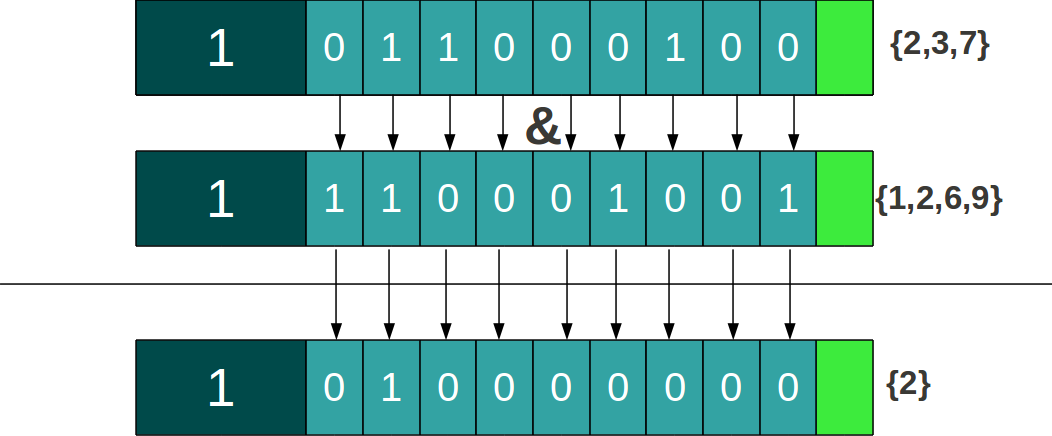
\includegraphics[height=50mm, scale=.5]{intersection.png}
\caption{Intersection operation achieved by AND-ing two BitVectors}
\end{center}
\end{figure}

\subsection{Implementation details of Difference $(-)$operation}
\ \ \ \ The figure 5 illustrates how \textit{\textbf{set difference}} operation is implements in textit{O(1)} using BitVectors by \textit{ANDing} first BitVector with the \textit{Complement} of second BitVector. \textit{Set difference} of two sets would result in a set that includes elements from the first set which are not present in the second set. To achieve \textit{Set difference} we need one \textit{AND} and one \textit{complement} operation. 
\begin{figure}[H]
\begin{center}
\ \newline
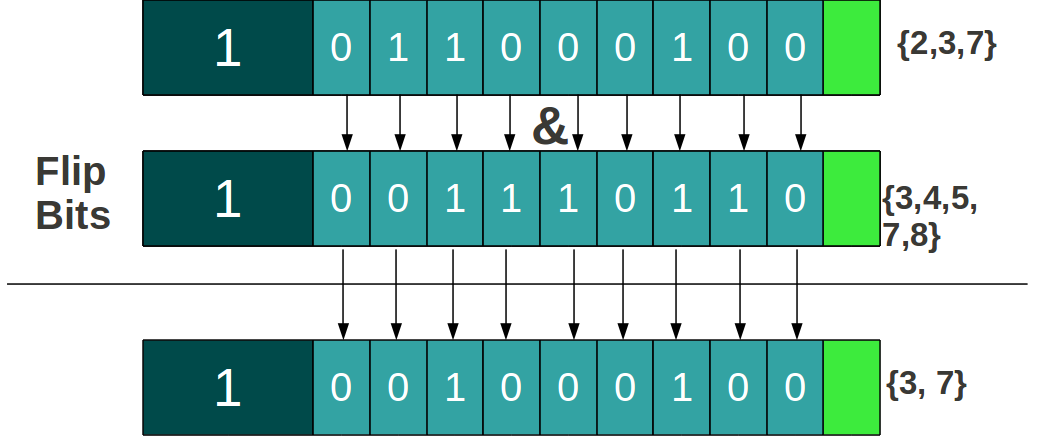
\includegraphics[height=50mm, scale=.5]{difference.png}
\caption{Set difference operation achieved by AND-ing first BitVector with complement of second BitVector}
\end{center}
\end{figure}


\section{Chapter : System Design and Implementation}
\ \ \ \ The System Design emphasizes on four techqniques using which the sudkoku is solved. each of the technique is discussed in the System design section. The four techniques to fill the cells of a sudodku are \textit{Basic Fillling, Elimination technique, Row and Column Analysis}. Each of the above techniques will be discussed in detailin System Design section. 

\subsection{Tools and Technologies used}
\subsubsection{Languages Used}
\begin{itemize}
\item{ C++ (Back end)}
\item{ Java (Front end) Swings}
\end{itemize}

\subsubsection{Tools Used}
\begin{itemize}
\item{ \LaTeX (LaTeX for reporting)}
\item{ OpenOffice (for presentation)}
\item{ sudoku (terminal version of Sudoku) }
\end{itemize}
\ \ \ \ Implementation of \textit{BitVector} data structure and associated \textit{SET} operations are implemented in \textit{C++}. The front end (\textit{GUI}) is implemented in \textit{Java Swings}. Java program calls the C++ program and gives the unsolved sudoku as input. The C++ program dumps the solution to a text file. Java then parses that text file and stores them in the \textit{solution string}. When Java GUI is asked to solve the Sudoku automatically then it uses that \textit{solution string} to show solution to the sudoku in GUI. GUI also includes features for user to solve on his/her own combined with auto solver. A count down timer is provided to count the time taken to solve the Sudoku. User is provided controls to pause/resume the auto solver and also to clear the current sudoku to start from the beggining (clear the entries made by the user).

\subsection{System Design}
\ \ \ \ System Design as specified earlier concentrates on four techniques for solving sudoku. Each of the four techniques are independent and execute on their own, but solutions from each technique will help other techniques to determine values to the remaining unfilled cells. Each of the four techniques are dependent on the \textit{\textbf{PosssibleValues}} of each of the cell. In understanding the algorithm certains variables and Data structures need to be understood and are explained below.\\
\ \newline
\textit{\textbf{Set}} -\ \ \ \ \ \ \ \ \ \ \  defines the Set Data Structure and its associated operations.\\
\textit{\textbf{cells[n][n]}} - defines the 9x9 grid cells.\\
\textit{\textbf{row[i]}} -\ \ \ \ \ \ \ defines row `i' (A set)\\
\textit{\textbf{column[i]}} - \ defines column `i'(A Set)\\
\textit{\textbf{box[n]}} - \ \ \ \ \ \ defines the 3x3 grid.\\
\textit{\textbf{cells[i][j].PossibleValues}} - define the possible values which might come in the cell. \\
\textit{\textbf{box[n].cells[i]}} - defines the cell \textit{`i'} in the box \textit{`j'}\\


\subsubsection{Defining PossbleValues of a Cell}
\ \ \ \ \textit{\textbf{PossibleValues}} of a cell is also a Set containing the possible values of a sudoku cell. Possible Values of a cells is defined as set of values which are not there in the row, column and box, where the cell exists. Possible Values of a cell is defined mathematically as\\
\ \newline
Let \textit{\textbf{C}} = \{ 1,2,3, . . ,9\}\\
$\forall \ \  0 \leq i, j \leq 8$ \\
$cells[i][j].PoossibleValues = C - ( row[i] \ \bigcup \ column[j] \ \bigcup \ BOX(boxval(i,j))\ )$\\
where,
$boxval(i,j)= (\lfloor i/3 \rfloor)*3 + (\lfloor j/3 \rfloor)$

\subsubsection{Basic Filling}
\ \ \ \ \textit{Basic filling} is a filling technique where a cell is filled with a value if the cardinality of the set PossibleValues is equal to one. In other words  If the cell can have only one value then just fill it. i.e. if $\vert PossibleValues \vert $= 1 then fill that cell with PossibleValue. \\

\subsubsection{Filling by Elimination}
\ \ \ \ In \textit{Filling by Elimination} technique, a cell \textit{`c'} of a box \textit{`b'} is filled with a value \textit{`x'} if \textit{`x'} is not a Possible Value in any of the other cell in the same box. i.e. A cell in a box is filled with a value if it cannot appear in any other cell in the same box. Filling By elimination can be mathematically defined as \\

if a cell \textit{`j'} is under consideration in the box \textit{`i'}\\

$Result = box[i].cell[j].PossibleValues - \bigcup\limits_{q=0}^8 box[i].cell[q].PossibleValue, where\  q \neq j$

if $\vert$Result$\vert$ = 1 then cell[j]=Result

\subsubsection{Filling by Row and column Analysis}
\ \ \ \ This to \textit{Filling by elimination}, but instead of applying the technique to a box, it is applied to row and column. Each row and column is scanned for cells which satisfy the criteria to fill the cells. 
\ \newline
\ \newline
\textbf{Row Analysis}\\
\ \ \ \ In \textit{Filling by Elimination} technique, a cell \textit{`c'} of a row \textit{`r'} is filled with a value \textit{`x'} if \textit{`x'} is not a Possible Value in any of the other cell in the same row. i.e. A cell in a box is filled with a value if it cannot appear in any other cell in the same row. Filling By row analysis can be mathematically defined as\\

if a cell \textit{`j'} is under consideration in the row \textit{`r'}\\

$Result = cell[r][j].PossibleValues - \bigcup\limits_{q=0}^8 cell[r][q].PossibleValue, where\  q \neq j $

if $\vert$Result$\vert$ = 1 then cell[r][j]=Result

\ \newline
\textbf{Column Analysis}\\
\ \ \ \ In \textit{Filling by Elimination} tehnique, a cell \textit{`c'} of a column \textit{`l'} is filled with a value \textit{`x'} if \textit{`x'} is not a Possible Value in any of the other cell in the same column. i.e. A cell in a box is filled with a value if it cannot appear in any other cell in the same Column. Filling By column analysis can be mathematically defined as\\

if a cell \textit{`j'} is under consideration in the row \textit{`l'}\\

$Result = cell[j][l].PossibleValues - \bigcup\limits_{q=0}^8 cell[q][l].PossibleValue, where\  q \neq j $

if $\vert$Result$\vert$ = 1 then cell[j][$l$]=Result

\subsection{System Implementation}
\ \ \ \ Implementation is done is two different languages. Front end in \textit{Java Swings}  and back end in \textit{C++}. The four techniques discussed in the previsous section are applied iterratively until solved. The \textit{Basic Filling} is applied to all the cells iterratively. If none of the cells are solved with this technique we go for the next technique (\textit{Fillin by Elimination}) else we will repreat the same technique. And the same applies for other three techiniques. If none of them were able to solve even one of the cell, then it is decided that the sudoku cannot be solved without guess. As explained earlier all these four techinques are independent of each other and they won't call each other. But output of one technique will be helpful for other techniques to determine values further. 

\subsubsection{Algorithm}
\ \ \ \ In the algorithms discussed below operator use `+' for union, `-' for Set difference operation and it is a sudo code. i.e. it is not a source code of any language. Some of the simple function are not shown here such as \textit{setValueAt(i,j,k)} means that set value `k' to \textit{cell[i][j]}, \textit{getUnion(i,j)} means that get the union of possible values of other cells in the same box except the cell cell[i][j]. 
\begin{flushleft}
\verb%filter()%
\\* \verb%{%
\\* \verb%  for(i=0 to 8)%
\\* \verb%    for(j=0 to 8)%
\\* \verb%      cell[i][j].PossibleValues = {1,2., .. 9} - %
\\* \verb%                                  (row[i] + column[j] + BOX(i,j))%
\\* \verb%}%
\end{flushleft}

\ \ \ \ The above algorithm is for generating possible values of all cells.

\begin{flushleft}
\verb%SolveSudoku()%
\\* \verb%{ do%
\\* \verb%  {   do%
\\* \verb%      {      n=0%
\\* \verb%             n=BasicFilling()%
\\* \verb%      }while(n>0)    %
\\* \verb%      do%
\\* \verb%      {      m=0%
\\* \verb%             m=FillByElimination()%
\\* \verb%      }while(m>0)    %
\\* \verb%      do{    o=0%
\\* \verb%             o=RowAndColumnAnalysis()%
\\* \verb%      }while(o>0)    %
\\* \verb%      if(n=0 AND m=0 AND o=0 ) then%
\\* \verb%      {      print("Sudoku Cannot be solved Without Guess")%
\\* \verb%             return 0%
\\* \verb%      }%
\\* \verb%  } while ( Sudoku not solved )%
\\* \verb%  return 1%
\\* \verb%}%
\end{flushleft}
\ \ \ \ This algorithm applies all the four techniques iterratively through all the cells. It keeps on solving sudoku in one technique. If that technique fails then moves for the next technique. If the last technique cannot determine further then again the first technique is started. If none of them were able to solve even a single cell then it it determined that sudoku is not solvable without guess and terminates.

\begin{flushleft}
\verb%FillByElimination()%
\\* \verb%{  count=0;%
\\* \verb%    for(i=0 to 8)%
\\* \verb%      for(j=0 to 8)%
\\* \verb%      {   if( cell not filled)%
\\* \verb%          {   temp=cells[i][j].PossibleValues%
\\* \verb%              temp =  temp -  getUnion(i,j)%
\\* \verb%              if( |temp| = 1)%
\\* \verb%              {   setValueAt(i,j,k)%
\\* \verb%                  count++%
\\* \verb%              }%
\\* \verb%          }%
\\* \verb%      }%
\\* \verb%        return count%
\\* \verb%}%
\end{flushleft}
\ \ \ \ \ The above algorithm determines value of cells using Elimination technique.
\begin{flushleft}
\verb%BasicFilling()%
\\* \verb%{   count=0;%
\\* \verb%    for(i=0 to 8)%
\\* \verb%       for(j=0 to 8)%
\\* \verb%       { if(cells[i][j].value == 0)%
\\* \verb%            if( |cells[i][j].PossibleValues|= 1)%
\\* \verb%            {  setValueAt(i,j,k)%
\\* \verb%               count++%
\\* \verb%            } %
\\* \verb%       }%
\\* \verb%    return count;%
\\* \verb%}%
\end{flushleft}
\ \ \ \ \ The above algorithm determines value of cells using Basic filling technique.
\begin{flushleft}
\verb%fillUsingRowColumnAnalysis()%
\\* \verb%{   n=0;%
\\* \verb%     for(i=0 to 8)%
\\* \verb%     { value=0%
\\* \verb%       Set currentRow=rows[i],temp=Set(1,2,..,9), temp2%
\\* \verb%       temp= temp-currentRow%
\\* \verb%       while((value=temp.getNextElement()))%
\\* \verb%         for(j=0 to 8)%
\\* \verb%           if( cells[i][j] to be filled)%
\\* \verb%             if(cells[i][j].PossibleValues.search(value)= found)%
\\* \verb%               {  temp2=cells[i][j].PossibleValues - getRowUnion(i,j)%
\\* \verb%                  if( |temp2| = 1)%
\\* \verb%                  {    setValueAt(i,j,temp2)%
\\* \verb%                       n++%
\\* \verb%                  }%
\\* \verb%              }%
\\* \verb%     }%
\\* \verb%     for(j=0 to 8)%
\\* \verb%     { int value=0%
\\* \verb%       Set currentColumn=columns[j],temp=Set(1,2,..,9), temp2%
\\* \verb%       temp= temp-currentColumn%
\\* \verb%       while((value=temp.getNextElement()))%
\\* \verb%         for(int i=0 to 8) %
\\* \verb%           if(cells[i][j] to be filled)%
\\* \verb%             if(cells[i][j].PossibleValues.search(value)= found)%
\\* \verb%               {  temp2=cells[i][j].PossibleValues - getColumnUnion(i,j)%
\\* \verb%                  if( |temp2| = 1)%
\\* \verb%                  {   setValueAt(i,j,temp2)%
\\* \verb%                       n++%
\\* \verb%                  }%
\\* \verb%               }%
\\* \verb%     }%
\\* \verb%    return n%
\\* \verb%}%
\end{flushleft}
\ \ \ \ The above algorithm determines value of cells using both row and column analysis 
\ \newline
\subsubsection{Snapshots}
\ \ \ \ The figure 6 shows the empty sudoku where all the cells are empty. We can see a drop down menu which has different levels of difficulties such as \textit{Easy}, \textit{Medium}, \textit{Hard} and \textit{Very Hard}. The generate button would generate a sudoku depending upon the selection in the difficulty drop down menu. Time taken to solve the sudoku is also shown. The button \textit{SolveAutomatically}, \textit{Pause} and  \textit{Stop} are disabled initially. When a sudoku is generated, \textit{SolveAutomatically} button and clear is enabled. When \textit{SolveAutomatically} button is clicked the GUI automatically starts solving the sudoku and \textit{Pause} button is enabled. When the entire sudoku is solved a popup will appear showing that sudoku is solved.
\begin{figure}[H]
\begin{center}
\ \newline
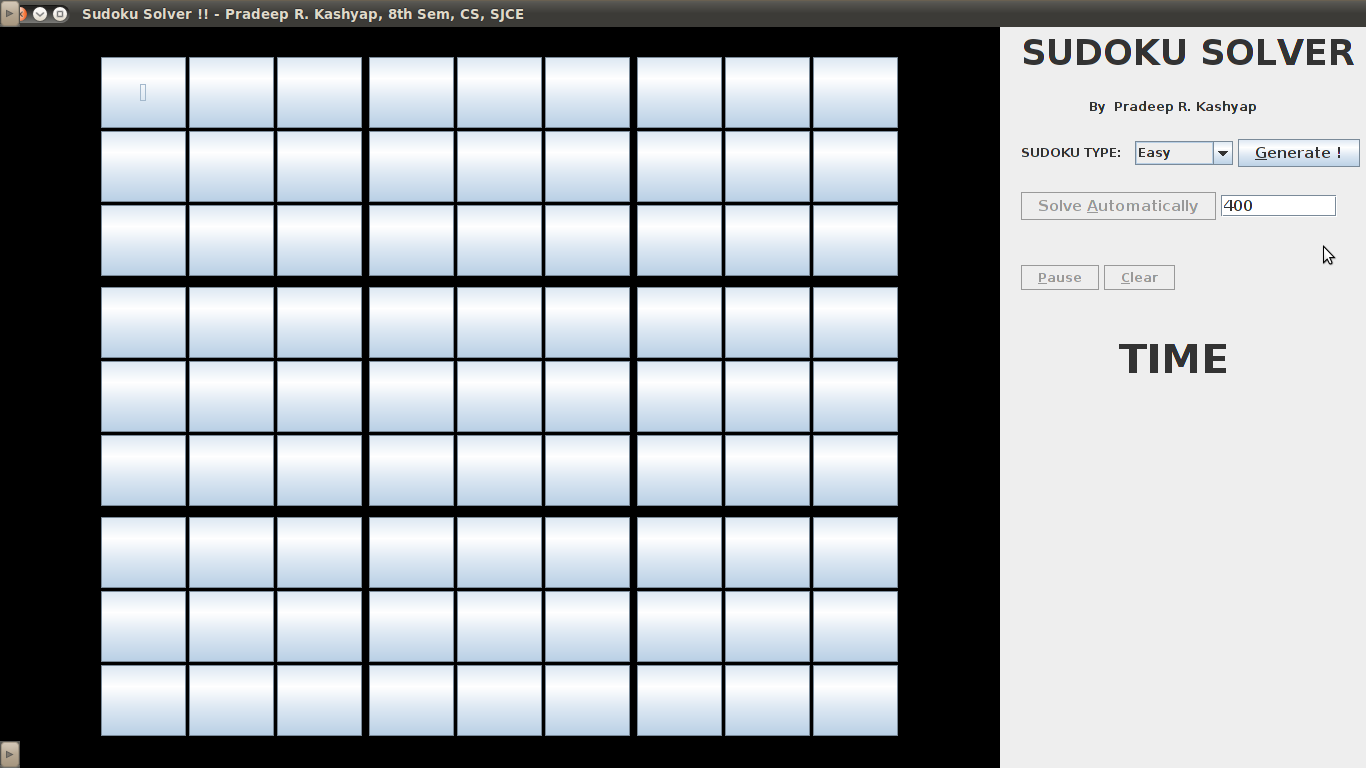
\includegraphics[height=75mm, width=150mm]{emptysudoku.png}
\caption{This figure shows the Empty Sudoku }
\end{center}
\end{figure}


\ \ \ \ When \textit{SolveAutomatically} is clicked the \textit{Solution String} stored is used to solve sudoku in GUI. The solution string is calculated at the time of generation of a sudoku. A text box is provided to give in the delay in how fast the computer should solve the sudoku. The \textit{Pause} button is used to pause the automatic solving. \textit{Clear} Button can be used to clear all the user made entries takes the sudoku to the inital state of the current problem. As as when the \textit{Generate} button is clicked the counter starts ticking and when the sudoku is completed, it stops.
\begin{figure}[H]
\begin{center}
\ \newline
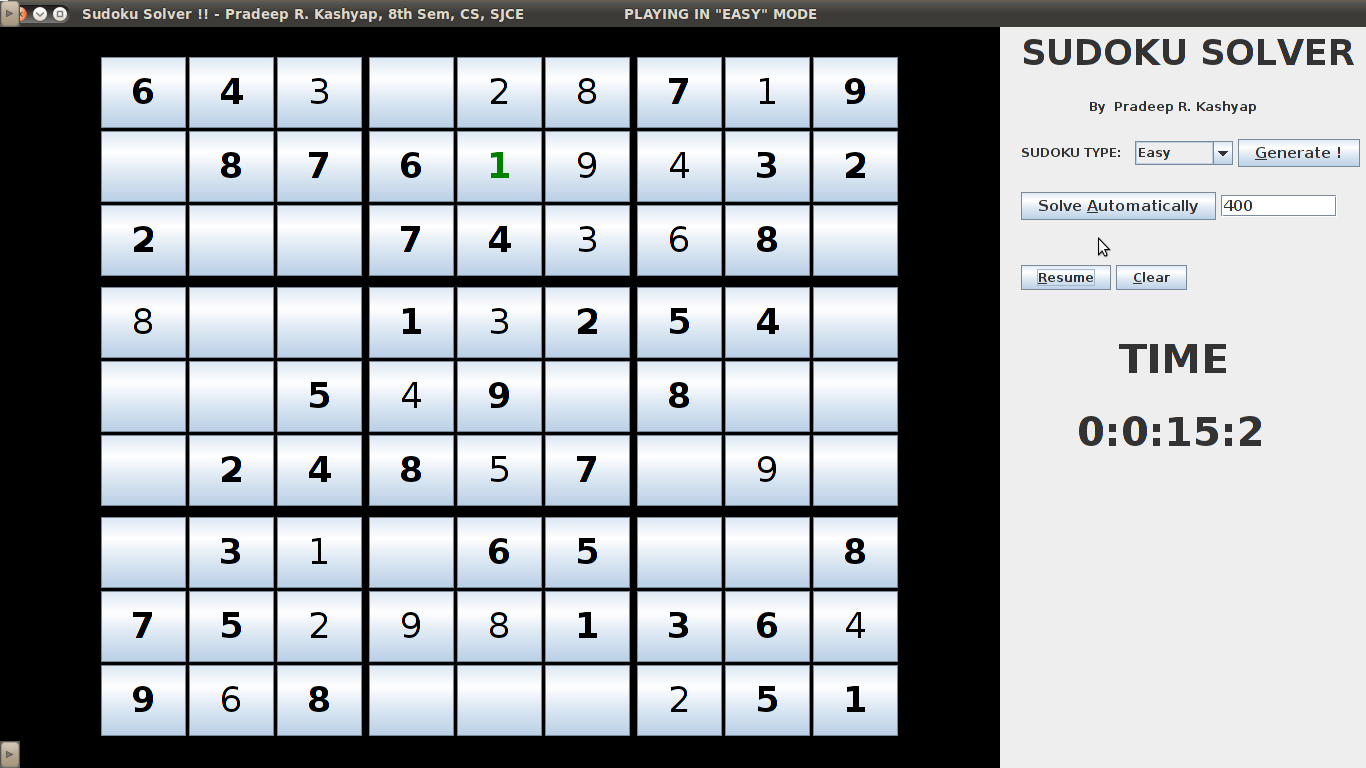
\includegraphics[height=75mm, width=150mm]{solveautomatically.png}
\caption{This figure shows GUI when SolveAutomatically Button is clicked }
\end{center}
\end{figure}

\ \ \ \ Sudoku can be solved using both \textit{SolveAutomatically} button as well as the user can give in the solution. A cel can be filled by taking the control on to that cell and typing the value to be placed. When all the cells are filled without any conflicts.
\begin{figure}[H]
\begin{center}
\ \newline
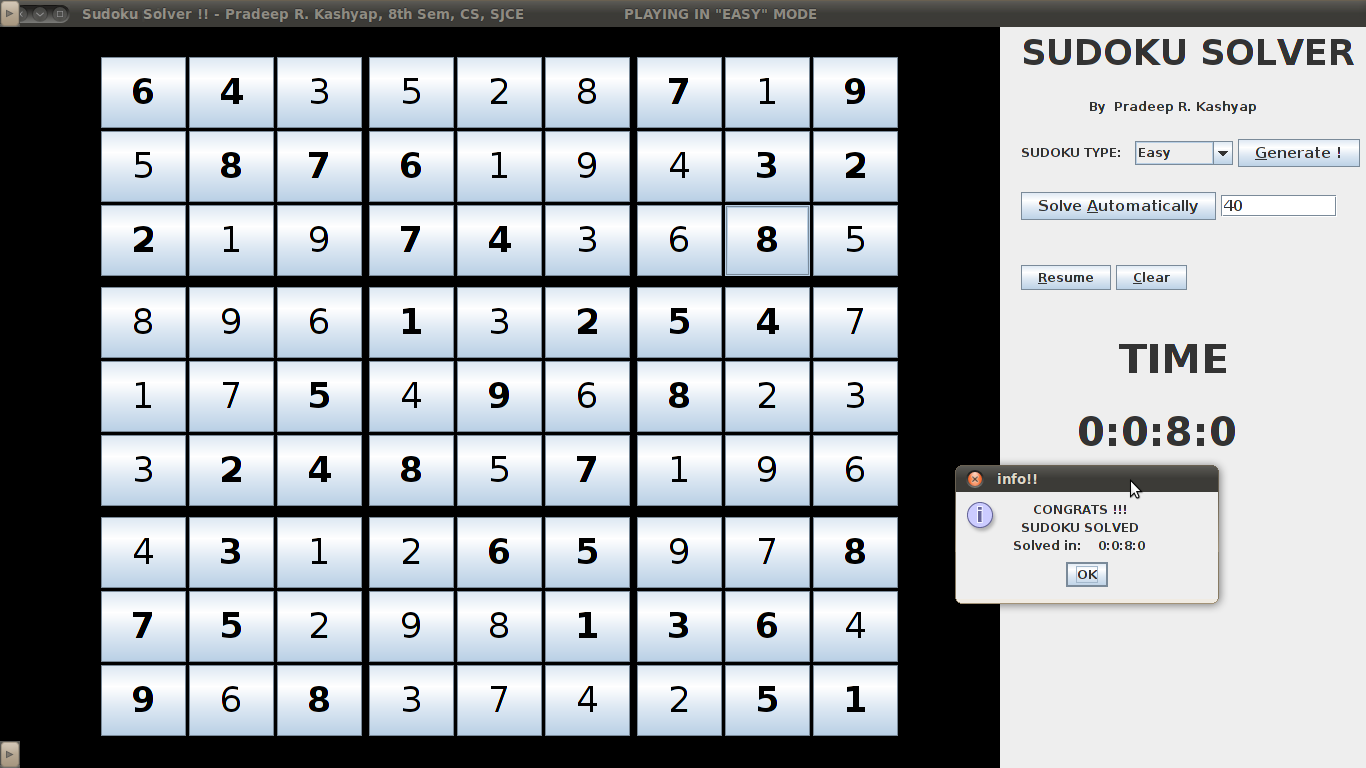
\includegraphics[height=75mm, width=150mm]{completed.png}
\caption{This figure shows the state of GUI when sudoku is completely solved.}
\end{center}
\end{figure}
\newpage
\section{System Testing and Results}
\subsection{System Testing}
\ \ \ \ The System has been test for more that \textit{\textbf{1000}} test cases including all the difficulty levels. The System works perfectly and provides complete solution to all the sudoku's till \textit{Hard} level. The \textit{Very Hard} level sudokus are not solvable without guess. Every partial solutions for such sudokus are provided. The system has been implemented such that whenever a wrong entry is made in a cell it shows the error. Hence we can verify whether the given solution (Automated or Mannual) is correct or not.
\subsection{Results}
\ \ \ \ The technique discussed provides solution to the sudoku in O(n$^3$), where as other techniques give solution in O(n$^5$) (Brute force technique) and O(N$^n$) (for backtracking technique). The explaination for how O(n$^3$) is given below
\begin{center}
O(n$^2$x( 4(1)x(3n))) = O(n$^3$)
\end{center}
where n$^2$ is for each cell, 4(1) is for 4 techniques and 1 is order of 1 for set operations, 3n is for accessing cells in row, column and box.
where as brute force technique without Set Data Structure requires O(n$^5$) and is explained below
\begin{center}
O(n$^2$x( 4(n$^2$)x(3n))) = O(n$^5$)
\end{center}
where n$^2$ is for each cell, 4(n$^2$) is for 4 techniques and n$^2$ is order of set operations (general array implementation of sets), 3n is for accessing cells in row, column and box.


\section{Conclusions and Furture work}
\subsection{Conclusions}
\begin{itemize}
\item{A mathematical appraoach was given to solve sudoku.}
\item{Set operations are extensively applied and solutions are obatained.}
\item{The technique is able to decide whether a sudoku is solvable without guess or not}
\item{Implementation Set operations BitVector helped to reduce the order of set operations from O(n$^2$) to O(1).}
\item{This technique is efficeient interms of both space and time.}
\end{itemize}
\subsection{Future work}
\ \ \ \ The proposed algorithm works at its best and O(n$^3$) is the best optimizations currently available. Due to the reduction in the order of set operations, this algorithm is able to run in O(n$^3$). To improve the efficiency further any new algorithm introduced should be able to access log(n) cells and no new technique can have order less than that.


\newpage
\section{References}
\begin{itemize}
\item{ Discrete And combinatorial Mathematics,by Raplph P. Grimaldi}
\item{http://www.maths.tcd.ie/~dwilkins/LaTeXPrimer/WhiteSpace.html}
\item{http://www.artofproblemsolving.com/Wiki/index.php/LaTeX:Symbols}
\item{http://amath.colorado.edu/documentation/LaTeX/reference/figures.html}
\item{http://tex.stackexchange.com/questions/8625/force-figure-placement-in-text}
\end{itemize}

\end{document}

